\documentclass[11pt,a4paper]{article}
\usepackage[latin1]{inputenc}
\usepackage{amsmath}
\usepackage{amsfonts}
\usepackage{amssymb}
\usepackage{graphicx}
\usepackage{parskip}
\usepackage{hyperref}
\usepackage{wrapfig}
\usepackage{listings}
\usepackage{color}
\usepackage{hyperref}
\usepackage{csvsimple}
\usepackage[left=2cm,right=2cm,top=2cm,bottom=2cm]{geometry}
\usepackage[table]{xcolor}

\DeclareMathOperator*{\argmax}{arg\,max}

\definecolor{dkgreen}{rgb}{0,0.6,0}
\definecolor{gray}{rgb}{0.5,0.5,0.5}
\definecolor{mauve}{rgb}{0.58,0,0.82}

\lstset{
  language=Python,
  aboveskip=3mm,
  belowskip=3mm,
  showstringspaces=false,
  columns=flexible,
  basicstyle={\small\ttfamily},
  numbers=none,
  numberstyle=\tiny\color{gray},
  keywordstyle=\color{blue},
  commentstyle=\color{dkgreen},
  stringstyle=\color{mauve},
  breaklines=true,
  breakatwhitespace=true
  tabsize=4
}

\author{Kevin Gao, Matt Li, Ashvin Nair, Saavan Patel}
\title{WHS Machine Learning: Lessons Learned}

%%%%%%%%%%%%%%%%%%%%%%%%%%%%%% Bibtex style
\usepackage{apacite} % http://www.ctan.org/tex-archive/biblio/bibtex/contrib/apacite/apacite.pdf
\bibliographystyle{apacite}

%%%%%%%%%%%%%%%%%%%%%%%%%%%%%% Document
\begin{document}

\maketitle

Introductory machine learning is the subject of a yearlong autodidactic pioneering computer-science course at Winchester High School. The intent of this course is to understand the algorithms of machine learning and implement them in code. In this course we studied decision trees, genetic algorithms, hidden Markov models, and artificial neural networks. Whenever possible, we applied the algorithms to real-world data.

The purpose of this paper is to publicize simple implementations of introductory machine learning algorithms in an accessible and clear way. For additional reference, our implementation of the below algorithms can be found at \url{https://github.com/anair13/whs-machine-learning}.

This work was completed at Winchester High School under the supervision of computer-science teacher \href{http://winchester.k12.ma.us/~dpetty/}{David C. Petty}.

\section{Decision Trees}
\label{DecisionTrees}

Decision trees use data to make predictions. Their purpose is to produce an answer while asking as few questions as possible, which is done by figuring out the most informative question at every point. This quickly narrows down the information into a likely answer.

\subsection{Data}
\label{DecisionTrees:Data}

For reference, we create a set of variables called attributes consisting of a name and possible values represented by the range from 0 to (number of values - 1). These attributes act as questions to ask about. For example, an attribute named ``temperature'' may have the values ``hot,'' ``mild,'' and ``cool'' or $\{0, 1, 2\}$. Most of the attributes are determining factors, but the very last attribute is the outcome, such as ``play tennis'' with values of ``yes'' or ``no.'' The value must be given when training the model, but it can be predicted from the other attributes once the model is constructed. The data itself is a matrix with each row being a separate case and each column containing values for an attribute. We get the information from a text file of the same format, gather all the values that appear for each attribute, assign them numbers, and finally parse the data into a two-dimensional array.

\subsection{Construction}
\label{DecisionTrees:Construction}

In the decision tree, the nodes contain an attribute and each of their branches is one of the attribute's values. The problem is to determine which attribute should be at each node. First the ``best question'' is asked, and the attribute is placed at the root of the tree. The values of the attribute each correspond to a branch, which leads to another question.

To decide on this ``best question'' we define the informational entropy $H(X)$ of a set $X$ as 

\[
H(X) = \sum{(-p^+ \log_2{p^+} - p^- \log_2{p^-})}
\]

where $p^+$ is the proportion of positive examples, and $p^-$ is the proportion of negative examples in the set.

Using $H(X)$, the information gain of a given question acting on set $A$ is

\[
H(A) - \sum_V{\frac{|Set V|}{|Set A|}H(V)}
\]

where the sum iterates through every set of positive examples $V$ (the different sets the question splits the data into). The ``best question'' is the attribute with the highest information gain.

This process is continued, deciding what to ask next based on the answer to each previous question, until a threshold is reached where the outcome can be determined with sufficient confidence.

\subsection{Usage} 
\label{DecisionTrees:Usage}

To create the tree, we use Node objects to represent each node of the tree. The objects contain one attribute and have children nodes. We use the algorithm with the original data to find the first question and place the attribute at the root node. For each of the attribute's values, we comb through the data and find only the cases with the same value for the attribute and create a new data set with the attribute removed. The algorithm is used again on the new data to figure out the next question. This attribute is then put into the child node for that value. The tree is grown recursively until we can predict the outcome with 95\% certainty.

For our ``playtennis'' problem, we have attributes as follows:

{
\begin{wraptable}{r}{3.5cm}
\begin{tabular}{| c | c | c | c | c |}
\hline
\rowcolor[RGB]{255, 150, 150}
0 & \cellcolor{white}0 & 0 & 1 & 0 \\ \hline 
\rowcolor[RGB]{255, 150, 150}
0 & \cellcolor{white}0 & 0 & 0 & 0 \\ \hline 
\rowcolor[RGB]{150, 255, 150}
0 & \cellcolor{white}1 & 0 & 1 & 1 \\ \hline 
\rowcolor[RGB]{150, 150, 255}
1 & \cellcolor{white}2 & 0 & 1 & 1 \\ \hline 
\rowcolor[RGB]{150, 150, 255}
2 & \cellcolor{white}2 & 1 & 1 & 1 \\ \hline 
\rowcolor[RGB]{150, 150, 255}
2 & \cellcolor{white}2 & 1 & 0 & 0 \\ \hline
\rowcolor[RGB]{150, 255, 150}
2 & \cellcolor{white}1 & 1 & 0 & 1 \\ \hline 
\rowcolor[RGB]{255, 150, 150}
1 & \cellcolor{white}0 & 0 & 1 & 0 \\ \hline 
\rowcolor[RGB]{255, 150, 150}
2 & \cellcolor{white}0 & 1 & 1 & 1 \\ \hline 
\rowcolor[RGB]{150, 150, 255}
1 & \cellcolor{white}2 & 1 & 1 & 1 \\ \hline 
\rowcolor[RGB]{255, 150, 150}
1 & \cellcolor{white}0 & 1 & 0 & 1 \\ \hline 
\rowcolor[RGB]{150, 255, 150}
1 & \cellcolor{white}1 & 0 & 0 & 1 \\ \hline 
\rowcolor[RGB]{150, 255, 150}
0 & \cellcolor{white}1 & 1 & 1 & 1 \\ \hline 
\rowcolor[RGB]{150, 150, 255}
1 & \cellcolor{white}2 & 0 & 0 & 0 \\ \hline 
\end{tabular}
\end{wraptable}

\begin{lstlisting}

ATTRIBUTES = [
Attribute("temperature", [0,1,2]), # ["hot","mild","cool"]
Attribute("outlook", [0,1,2]), # ["sunny","overcast","rainy"]
Attribute("humidity", [0,1]), # ["high","normal"]
Attribute("wind", [0,1]), # ["strong","weak"]
Attribute("playtennis", [0,1]), # ["no","yes"]
]
\end{lstlisting}

On the right is the data. After determining that outlook is the best question to ask first, we group the data based on the value for outlook. Since we do not want to ask the same question again, the data for outlook is removed. The red cells become the data used to decide the question for the node at the ``sunny'' branch, green for the ``overcast'' branch, and blue for the ``rainy'' branch.

\newpage
\subsection{Results}
\label{DecisionTrees:Results}
}

We applied the decision tree program to car buyers, the census, congressional voting records, and CPU performance data. It was usually able to give a confident answer within just a handful of questions out of a dozen or more attributes. This varied greatly with the strength of association between attributes and whether the specific case followed the trends of others.

The tree itself starts with a question and asks another question for each possible answer until it predicts an outcome. This is the tree we created from congressional voting records.

{
\ttfamily
el-salvador-aid? \\
| y--education-spending? \\
| | y--physician-fee-freeze? \\
| | | y--aid-to-nicaraguan-contras? \\
| | | | y--republican \\
| | | | n--democrat \\
| | | n--religious-groups-in-schools? \\
| | | | y--republican \\
| | | | n--democrat \\
| | n--republican \\
| n--democrat
}

We used Weka to check our results, and our trees were almost identical to theirs, with small differences in the level of pruning based on the threshold we used for certainty.

\subsection{Conclusion}
\label{DecisionTrees:Conclusion}

Decision trees are an efficient way to crunch a lot of information down to a few key questions that can fairly accurately predict an outcome. While it becomes harder to use when the number of attributes becomes extremely large, its advantage over many other predicting algorithms is that it requires less instances of data to create a useful model. The simple structure of the decision tree makes it a great introduction to machine learning.

\section{Genetic Algorithms}
\label{Genetic Algorithms}

Genetic algorithms find parameters to optimize a given function. We used it in combination with the Hungarian algorithm to create a program that selects an optimal math team given individual mathlete scores. In this section, we explain our implementation of a genetic algorithm, as well as explain our larger program.

The genetic algorithm is a computational implementation of the theory of natural selection in nature. The idea behind the algorithm is ``survival of the fittest,'' where the fittest individuals are the most likely to survive to the next generation. The idea of mutations is also introduced, where random mutations occur within the population that introduce variability, and reduce the chances of the population being stuck in a local maxima, when global maxima are available.

\begin{figure}[h]
  \begin{center}
	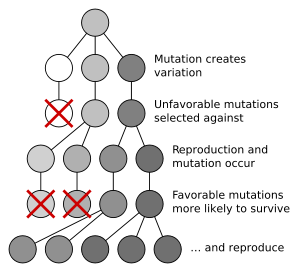
\includegraphics[scale=0.6]{natural_selection.png}
  \end{center}
  \caption{A simple description of the theory behind natural selection}
\end{figure}

\subsection{Data}
\label{Genetic Algorithms:Data}

Genetic algorithms attempt gradient ascent of parameters by mimicking natural selection. Given a fitness function to be optimized, an individual is defined as a set of parameters for the function and we call each parameter an ``attribute" of that individual.

\subsection{Construction}
\label{Genetic Algorithms:Construction}

Generally, a genetic algorithm optimizes a function with a large set of parameters when the result of a parameter change is unknown. To start a genetic algorithm, a population,$N$, of random individuals with random traits is generated. Each individual represents a set of parameters to be optimized. The goal is to generate a population of almost homogeneous individuals that all represent the fittest possible member of the population.

Fitness (the fitness of individual $I$ will be denoted $F_{I}$) is a function that measures the success of the individual: higher fitness means that the individual is more likely to reproduce.

In addition, the algorithm depends on:
\begin{itemize}
\item Crossover rate $C$, the probability a trait is crossed over during breeding
\item Mutation rate $M$, the probability that a trait is randomly changed. Mutations are used to prevent individuals from converging at local extrema and therefore miss global extrema.
\item Breed proportion $B$, the proportion of each population that is generated from ``children'' of individuals in the previous population
\end{itemize}

In all, the total process runs:

\begin{enumerate}
\item An individual is selected based on its fitness, the probability is:

\[
P(I) = \frac{F_{I}}{\sum{F}}
\]

\item The individual is either set to breed or put directly into the next generation, depending on $B$.
\item If the individual is set to breed, another individual is selected with probability $P(I)$. ``Breeding'' occurs when two new individuals are created by switching random traits between the two individuals. $C$ is the probability one of the traits is switched between individuals. In this way, two new individuals become part of the new population.
\item Individuals are selected from the previous population with probability $P(I)$ and put directly into the next generation
\item Before individuals enter the next generation, traits may be mutated with a probability $M$. 
\end{enumerate}

The above process is repeated until a set number of generations has occurred or until a specific constraint has been met.

In code, the creation of a new generation looks like the following (note the binary search function \verb|bisect_left| to optimize choosing individuals):

\begin{lstlisting}
for ind in self.population:
   rand = random.random()
   if rand < self.MUTATION:
       # creates part of new population using mutations of random individuals
       new_pop.append(self.mutate(ind))
   elif rand < self.MUTATION + self.BREED:
       # creates part of new population using crossovers based on weights
       rand1 = random.random() * total_fitness
       rand2 = random.random() * total_fitness
       parent1 = self.population[bisect_left(weights, rand1)]
       parent2 = self.population[bisect_left(weights, rand2)]
       new_pop.append(self.breed(parent1, parent2))
   else:
       # fills the rest of the population based on weights of individuals
       rand = random.random() * total_fitness
       new_pop.append(self.population[bisect_left(weights, rand)])

self.population = new_pop
\end{lstlisting}
\subsection{Usage}
\label{Genetic Algorithms:Usage}

Data was presented in the form of a csv file containing the individual scores of the 20 math team members for a try out. The goal was to choose 10 members out of the 20, each member competing in 3 out of the 5 rounds available. The csv file contains the score for each of the math team members and the score for each of the 5 rounds.

Genetic algorithm for math team selection was combined with the Hungarian algorithm to efficiently produce a result. The genetic algorithm produced a team, and the Hungarian algorithm chose which members of the team would do which rounds, which in turn went to the fitness algorithm, which calculated the fitness of the given team (the total score of the team).

\subsubsection{Hungarian Algorithm}
\label{Genetic Algorithms:Hungarian Algorithm}

We implemented the Hungarian algorithm as a part of the fitness algorithm in math team selection. The Hungarian algorithm solved the optimization problem in polynomial time, which makes the rest of the genetic algorithm more efficient.

The algorithm takes an $N \times N$ matrix of numerical values and returns $N$ values such that one is chosen from each row and each column and the sum of the values is maximized. Starting with the first row, it searches through every column to find the highest value in the row. The process is repeated with the second row. If the values have been selected from different columns, the algorithm proceeds to the next row. Once a conflict is found, the two rows with maximum values in the same column are searched again for the second highest values. The two possible combinations are compared and the one that produces a higher sum is chosen. (In the case that the sums are equal, the choice can be made arbitrarily as they will produce equally maximized solutions.) If this creates another conflict, it is resolved similarly, potentially looking at third highest values, fourth highest values, and so on until the solution is found.

Our math team problem consists of assigning ten members to three rounds each, with six rounds to choose from, and therefore five members performing in each round. We represent this with a 30 by 30 matrix so that each member appears three times and each round five times. Each member has a ``score'' for each round, collected from previous practices and tryouts. When running through the algorithm, once a member is selected for a round, the other fourteen elements of the matrix with the same member-round combination are lowered by a large arbitrary constant so that the member will not be chosen again for the same round.

\subsection{Results}
\label{Genetic Algorithms:Results}

A comma-separated-values file of the scores of approximately 20 math team members is entered into the algorithm, and optimal math teams are outputted through the command line. The algorithm works to pull a team of 10 math team members, and pick 3 out of the 5 available rounds for each math team member. In many cases, there are multiple optimal math teams. The algorithm is able to optimize for the math team problem within 100 generations, which takes approximately 1 minute to complete. This shows that the genetic algorithm in combination with the hungarian algorithm is effective in solving the math team allocation problem in an acceptable period of time, and could actually be useful in helping a real math team.

\subsection{Conclusion}
\label{Genetic Algorithms:Conclusion}

The genetic algorithm is a useful optimization tool when the effect of parameters on the overall fitness of a function is unknown. We learned the simplest optimization tool in the machine learning environment, and provided a base for further endeavors into the field. The genetic algorithm provides a useful base for more complex and efficient algorithms, such as simulated annealing. By combining the genetic algorithm with the Hungarian algorithm to solve a real problem our math team had, we found a great use for our programming and a useful way to combine otherwise unrelated algorithms.

\section{Hidden Markov Models} 
\label{Hidden Markov Models}

Hidden Markov model algorithms perform pattern recognition. A basic Markov chain refers to a sequence of states where the probabilities of the next state are only dependent upon the previous state. In a hidden Markov model, these states are not directly observable; instead, they emit observations. For example, a person may be in the state of being ``sick" or ``healthy", but this state is not observable; we must infer their state of health from the symptoms they exhibit. More rigorously, a hidden Markov model $\lambda$ outputs an observation sequence $O$ (the corresponding state sequence $Q$ is hidden) using the parameters:

\begin{itemize}
\item $S$, the set of states $\{S_1, S_2, ... , S_N\}$
\item $O$, the set of observations $\{O_1, O_2, ... , O_M\}$
\item $\pi$, a list of starting probabilities of each state (length $N$)
\item $A$, a matrix of transition probabilities from state to state (size $N \times N$)
\item $B$, a matrix of emission probabilities from state to observation (size $N \times M$) 
\end{itemize}

We are interested in solving three different problems about such sequences:
\begin{enumerate}
\item Find $P(O|\lambda)$, the probability of a specific observation sequence ocurring, given the model
\item Find the state sequence $Q$ that maximizes $P(Q|O, \lambda)$, the probability of a specific state sequence producing a certain observation sequence, given the model.
\item Find the model $\lambda$ that maximizes the probability of a given list of observation sequences. This allows us to generate these models.
\end{enumerate}

\subsection{Data}
\label{Hidden Markov Models:Data}

Hidden Markov models care about sequences of events. They can be applied to data like sentences with each word tagged with a part of speech, where the innate cause of the sequence is not known but the emission of nouns and verbs is easy to identify. In our testing, we generated sequences from models, then tested whether we could predict the underlying states of those sequences and generate precise models back from those sequences.

\subsection{Construction}
\label{Hidden Markov Models:Construction}

The problems are related but each method is separate. Probabilistic quantities overlap between the problems, but each problem can be neatly divided into its own solution.

\subsubsection{Problem 1: $P(O|\lambda)$}
\label{Hidden Markov Models:Problem 1}

To find the probability of a specific observation sequence ocurring, given the model, we recursively calculate the probability of each element of the observation sequence occurring. Define the ``forward'' function $\alpha(n, i ,O|\lambda)$ as the probability of the first n observations ocurring and $Q_n$ being $S_i$.

In the base case where n = 1, the probability of ending on a known state is simply the start probability, and the probability that single observation occurs from the state is the emission probability from $S_i$ to $O_1$.

\[
\alpha(1, i, O, \lambda) = \pi_i * B_{iO_1}
\]

Going forward, $\alpha$ is the sum iterating through every previous state:

\[
\alpha(n, i, O, \lambda) = B_{iO_{n-1}} \sum_j^S{\alpha(n - 1, j, O, \lambda)A_{ji}}
\]

Building up,

\[
P(O|\lambda) = \sum_i^S{\alpha(N, i, O, \lambda)}
\]

\subsubsection{Problem 2: $P(Q|O, \lambda)$}
\label{Hidden Markov Models:Problem 2}

To maximize $P(Q|O, \lambda)$ (find the best underlying state sequence), we will recursively find the best state sequence of increasing lengths until the length of the observations is reached. In the following explanation, we are operating under a given sequence of observations $O = \{O_1, O_2, ..., O_N\}$ and a given model $\lambda(A, B, \pi)$.

Let the function $C(q, n)$ return the best state sequence of length $N - n + 1$ accounting for observations $O_n$ to $O_N$, and $C_p$ be the probability of that sequence. We will start with $n = N$ and $q = \{Q_N\}$ and recurse backwards.

If $n = 1$, the length of $q$ is $N$; $C$ simply returns $q$ as the sequence is already created and the probability of the sequence ocurring and having generated the observations is the starting probability of $q_1$ and the emission of $O_1$ by $q_1$:

\[
C_p(q, 1) = C_p(q, 2) \pi_{q_1} B_{{q_1}{O_1}}
\]

The recursive step is to find the best state to add to the start of $q$:

\[
C(q, n) = q + \{\argmax_{s \in S} C_p(q + \{s\}, n - 1)\}
\]

The above is implemented as:

\begin{lstlisting}
def best_current_state(states, n, observations, hmm):
    state = states[0]
    if n == 1:
        return hmm.start[state] * hmm.emission[state][observations[0]], states
    best_score = 0
    ret_states = None
    for s in hmm.states:
        tmp = best_current_state([s] + states, n - 1, observations, hmm)
        score = tmp[0] * hmm.transition[s][state] * hmm.emission[state][observations[n - 1]]
        if score > best_score:
            best_score = score
            ret_states = tmp[1]
    return best_score, ret_states
\end{lstlisting}

The best state sequence for $O$ is $C(\{\}, N)$.

\subsubsection{Problem 3: $P(\lambda|\{O\})$}
\label{Hidden Markov Models:Problem 3}

Although there are many optimizations to this process, the simplest method to extract a model from observations is counting:
\begin{itemize}
\item $\pi_i$ is the count of the first state being $S_i$ divided by the total observations
\item $a_{ij}$ is the count of transitions from $S_i$ to $S_j$ divided by the occurences of $S_i$
\item $b_{ij}$ is the count of emissions from $S_i$ to $O_j$ divided by the occurences of $S_i$
\end{itemize}

To optimize, the first quantity we must define is the probability that $Q_n$ being $S_i$. That is, $P(Q_n = S_i | O, \lambda)$. To help us, we add to our tools the backward analog of the forward algorithm. Arbitrarily, we define

\[
\beta(N, i, O, \lambda) = 1 \\
\]

Then by a similar logic as the forward algorithm:

\[
\beta(n, i, O, \lambda) = B_{iO_{n+1}} \sum_j^S{\beta(n+1, j, O, \lambda)A_{ji}}
\]

Given some observations, the probability that the $n^{th}$ state is state $i$ is:

\[
P(Q_n = S_i) = \frac{\alpha(n, i) \beta(n, i)}{P(O|\lambda)}
\]

The probability of seeing the first $n$ observations and ending in $S_i$ is the forward term, the probability of seeing the rest of the observations and starting with $S_i$ is the backward term, and the observation is given so we divide by $P(O|\lambda)$. Using this function, we can incrementally improve the parameters of the model by gradient ascent.

\subsection{Conclusion}
\label{Hidden Markov Models:Conclusion}

Although we were not able to use the hidden Markov model algorithms with much real data, the predictive power of the models was evident. We could generate a model with given parameters, generate observation sequences from the model and accurately predict the underlying state sequences using the above algorithms. Working through the math and probability quantities were especially instructive in thinking about drawing inferences about sequential events.

\section{Artificial Neural Nets}
\label{Artificial Neural Nets}

\begin{wrapfigure}{r}{0.4\textwidth}
  \begin{center}
	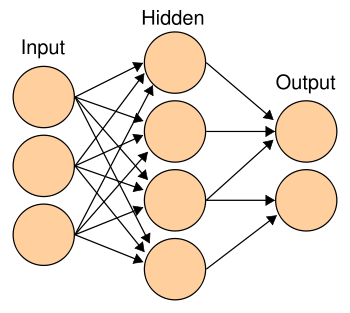
\includegraphics[scale=0.4]{neural_network.jpg}
  \end{center}
  \caption{A simple hidden network with three inputs, two ouputs, and one hidden layer}
\end{wrapfigure}

Artificial neural nets are a form of function approximation learning. They mimic the action of neurons: the output of each node is a function of the inputs from the previous layer. 

Each connection has a weight $w_{ik}$ that determines how much the input $x_i$ affects the output of the neuron.

An artificial neural network requires an input and output layer. One or more hidden layers act between the input and output layers. Each layer can have any number of neurons. 

Artificial neural networks are trained through the backwards propagation of errors. The goal of backwards propagation is to adjust the weights of the connections until the error between training example output and network output is at a minimum.

\subsection{Data}
\label{Artificial Neural Nets:Data}

Artificial neural networks attempt to approximate functions. That is, using a series of training examples, a list of inputs concatenated with corresponding outputs, the network adjust weights to resemble a probable function. Inputs and outputs can easily be mapped to real world quantities. For example, we represented pictures of letters as one hundred inputs.

\subsection{Construction}
\label{Artificial Neural Nets:Construction}

First, we must discuss the inner workings of a neural net. Each neuron passes its inputs through the sigmoid function:

\[
O_k(x, w) = \cfrac{1}{1 + e^{A(x, w)}} 
\]
where 
\[
A_k(x, w) = \sum_{i=0}^n{x_i*w_{ik}}
\]
$x$ is a list of inputs and $w$ is a matrix of connection weights.

\begin{wrapfigure}{l}{.4\textwidth}
  \begin{center}
	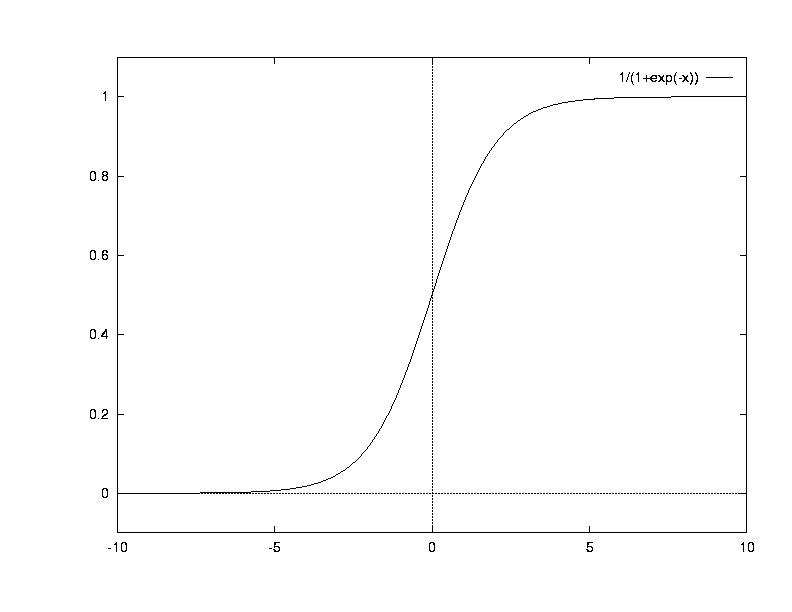
\includegraphics[scale=.3]{sigmoid.png}
  \end{center}
  \caption{The sigmoid function}
\end{wrapfigure}

We chose to use the sigmoid function -- $f(x) = \cfrac{1}{1 + e^x}$ -- as a continuous alternative to a simple step function, though the step function is also commonly used. $f$ is asymptotically close to 0 for large negative values, close to 1 for large positive values, and $f(0) = 0.5$.

The sigmoid function is also easily differentiable, which makes it easier to perform the backwards propagation algorithm. In particular $\frac{df}{dx} = f(1-f)$.

For a given list of inputs $x$, the input nodes output the value of itself. In other words, if one is the input to an input node, the input node will output 1. The inputs of each successive layer are calculated using the weights, and in the end the value of the output nodes are read.

To train the network, the general idea is to adjust weights until the error between training output and network output is minimized. We go forward through the network to find the output, then propagate errors backward and adjust each connection weight accordingly.

\begin{wrapfigure}{r}{0.5\textwidth}
  \begin{center}
	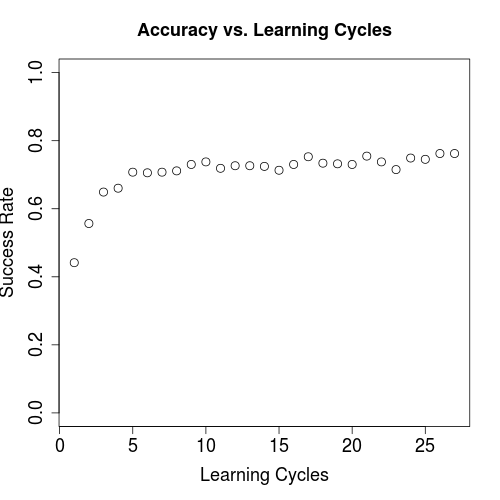
\includegraphics[scale=0.5]{graph.png}
  \end{center}
  \caption{Increasing learning cycles increases recognition accuracy, to a point}
\end{wrapfigure}

At the beginning random weights are assigned to all the connections. The weights of each neuron are adjusted a tiny amount by a single training example, and the network converges to the training behavior over time.


The backward error propagation begins with the error $\delta$ of each output node. We will call the list of inputs $x$, training outputs $o$, and outputs of the network currently $y$. The training example is run through once, and the output of each node $v$ is also saved. For the output nodes,

\[
\delta_i = o_i - y_i
\]

\begin{wraptable}{l}{.45\textwidth}
\csvautotabular{pr_lows.csv}
\vspace{-120px}
\end{wraptable}

For each node in the previous layer, the part of the error contributed by node $j$ to output node $i$ must be $w_{ji}$, so each node $j$ has

\[
\delta_j = \sum_i{\delta_i w_{ji}}
\]

In this way, every node in the network is updated with a value of $\delta$. Finally, we go forward through the network and adjust each weight:

\begin{gather*}
\frac{df}{de} = v_j (1 - v_j) \\
w_{ij} = w_{ij} + \eta \delta_i \frac{df}{de}v_i
\end{gather*}

where $\eta$ is a constant factor for learning rate (we set it at 0.1).

Repeatedly running each training example through the network will increase the precision of the network. In order to obtain reasonable results with even simple functions, we had to run the entire set of data through the network 30 times. Below, we have our success rate plotted with additional learning cycles of the data for our character recognition project.

\subsection{Usage} 
\label{Artificial Neural Nets:Usage}

In our implementation, each node is an object that saves its own last output. The network consists of a list of nodes, a matrix of weights, and a list of length of layers. To output, the nodes are iterated through layer by layer until the output nodes are calculated. Networks can be trained with training examples, and also saved and loaded to a persistent text file.

\begin{wraptable}{r}{.45\textwidth}
\vspace{-20px}
\csvautotabular{pr_caps.csv}
\csvautotabular{pr_nums.csv}
\caption{Precision, recall, and F-measure for each character identified}
\vspace{-70px}
\end{wraptable}

Our project includes a neural net for optical character recognition. Using a mouse or pen tablet one can write a letter or number and our neural net will guess the character.

From \citeA{web:chars-74k-hand-drawn} we found roughly 2000 sample images, 55 of each character, for our training examples. (These samples are avilable for study given that we cite \citeA{paper:deCampos09} as the original research.) In practice, we use 45 of each character to train and save 10 to test on. Using PIL, we crop each image into a square tightly containing the nonwhite regions of the image, then turn the images into 10x10 grayscale images. Each image is then represented as a list of 100 numbers: each pixel is converted into a number where white is -1 and black is 1. The output is a list of 62 numbers where each number represents a different character. The number corresponding to the correct character is 1 and the rest are 0. After training, the highest output corresponds to the letter predicted by the network.

Our network has a 100 input neurons connected to a hidden layer of 100 neurons. The hidden layer is then connected to 62 output neurons. This means there are 16200 connections, each of which has a weight that needs to be adjusted for each testing example. We also run the entire list of testing examples through the learning process 30 times in order to get better results.	

Once our network has been constructed we use a mouse or pen tablet to draw an image in our GUI. This image is converted into inputs the same way as the training examples. When the inputs are run through the network, each output neuron gives a value between 0 and 1 and the highest value is chosen as the predicted character.

\subsection{Results}
\label{Artificial Neural Nets:Results}

First, we tested our implementation with simple functions: given a number, return the number, its negative, and half of the number. As we ironed out the implementation, the neural net was extremely accurate in approximating these functions. We could define a neural network with our own parameters as a function to be approximated, and the training network would exactly replicate the given network within 1\% of each parameter given enough cycles through the data (In our case, 1000 cycles of 6 training examples through a network with 2 input, 2 hidden, and 2 output layers.)

Our optical character recognition has a 75\% success rate. As shown in the graph, when we run the data set through the first time, the success rate is only around 40\%. We believe that the 75\% success rate plateau is due to a lack of data, only 55 examples for each letter. Our character recognition seems to work far better on letters with straight lines such as T or A. This is probably because when we scale down, the letters with straight lines end up being more distinct. The character recognition also has difficulty with letters such as z, where people write it many different ways (with and without the line through the middle). It also makes expected errors such as 0 for o. Our construction process takes around 5 minutes when we run through 30 cycles of training data (the backwards propagation algorithm runs 58800 times). We are satisfied with the speed of training, since training does not need to be done in real-time and we are limited by the quantity of data.


\subsection{Conclusion}
\label{Artificial Neural Nets:Conclusion}

We found that neural networks are extremely efficient at sorting through large amounts of complicated data and finding the underlying function that we care about. However, they require a lot of data to be effective. In our case, increasing resolution of the image, and therefore increasing inputs, exponentially increases the amount of training time. On the whole, our lasting impression of neural networks is that they are an amazing tool to model convoluted functions given that we have a lot of data about the function.

\section{Conclusion}
\label{Conclusion}

The big picture we take away from this class is that by cleverly applying data to adjust parameters, machines can be trained to be really, really smart. We were taken aback by the complicated behavior: prediction, optimization, and character recognition, produced by a few simple lines of code combined with a large amount of data. Through our survey, we discovered that this field of applied statistics and computer science called machine learning is incredibly interesting. Besides the specific algorithms, we improved our implementation skills and learned new ways to think about handling and using data. We would highly recommend future classes with similarly free structure and topics.

\citeA{DBLP:journals/corr/cs-NE-0308031} and \citeA{book:pattern-classification} should force bibliography references.

%%%%%%%%%%%%%%%%%%%%%%%%%%%%%% Bibliography
\bibliography{mlbibtex} % To update, delete *.bbl

%%%%%%%%%%%%%%%%%%%%%%%%%%%%%% Index
%\printindex % To update, delete *.ind

\end{document}
